\documentclass{article} % For LaTeX2e
\usepackage{iclr-style/iclr2016_conference,times}
\usepackage{hyperref}
\usepackage{url}
\usepackage{amsmath}
\usepackage{amsfonts}
\usepackage{graphicx}
\usepackage{caption}
%\usepackage{subcaption}
\usepackage{subfig}
\usepackage{tabulary}
\usepackage{soul}
\usepackage{color}
\usepackage{xcolor}

\captionsetup{font=small}

\newcommand{\comm}[1]{}
\newcommand{\given}{\,|\,}
\newcommand{\expectation}{\mathbb{E}}
\newcommand{\kldiv}{\mathrm{D}_{\rm KL}}
\newcommand{\klBars}{\,\|\,}
\newcommand{\sigmoid}{\boldsymbol{\sigma}}
\newcommand{\hlang}{h^{lang}}
\newcommand{\hlangall}{\boldsymbol{h^{lang}}}
\newcommand{\hdec}{h^{dec}}
\newcommand{\henc}{h^{enc}}
\newcommand{\readop}{\mathit{read}}
\newcommand{\writeop}{\mathit{write}}
\newcommand{\encoder}{\mathit{LSTM}^{enc}}
\newcommand{\decoder}{\mathit{LSTM}^{dec}}
\newcommand{\canv}{c}
\newcommand{\lat}{z}
\newcommand{\Lat}{Z}
\newcommand{\numSamples}{L}
\newcommand{\sampleIdx}{l}
\newcommand{\LatSample}{\tilde{Z}}
\newcommand{\icaption}{{\bf{y}}}
\newcommand{\oimage}{{\bf{x}}}
\newcommand{\post}{Q}
\newcommand{\prior}{P}
\newcommand{\loss}{\mathcal{L}}
\newcommand{\lloss}{\mathcal{L}^{z}}
\newcommand{\rloss}{\mathcal{L}^{x}}
\newcommand{\hlc}[2][yellow]{{\sethlcolor{#1}\hl{#2}}}

\definecolor{0}{RGB}{247,251,255}
\definecolor{1}{RGB}{222,235,247}
\definecolor{2}{RGB}{198,219,239}
\definecolor{3}{RGB}{158,202,225}
\definecolor{4}{RGB}{107,174,214}
\definecolor{5}{RGB}{66,146,198}

\newcommand{\hlczero}[1]{\hlc[0]{#1}}
\newcommand{\hlcone}[1]{\hlc[1]{#1}}
\newcommand{\hlctwo}[1]{\hlc[2]{#1}}
\newcommand{\hlcthree}[1]{\hlc[3]{#1}}
\newcommand{\hlcfour}[1]{\hlc[4]{#1}}
\newcommand{\hlcfive}[1]{\hlc[5]{#1}}

\newcommand{\ssmall}[1]{{\scriptsize {#1}}}


\newenvironment{myfont}{\fontfamily{[pcr]}\selectfont}{\par}
\DeclareTextFontCommand{\textmyfont}{\myfont}

\setlength{\abovecaptionskip}{5pt} % Chosen fairly arbitrarily
\setlength{\belowcaptionskip}{5pt} % Chosen fairly arbitrarily

\title{Generating Images From Captions\\ With Attention}

\author{
Elman Mansimov, Emilio Parisotto, Jimmy Lei Ba \& Ruslan Salakhutdinov\\
Department of Computer Science\\
University of Toronto\\
Toronto, Ontario, Canada \\
\texttt{\{emansim,eparisotto,rsalakhu\}@cs.toronto.edu}, \texttt{jimmy@psi.utoronto.ca}
}

\newcommand{\fix}{\marginpar{FIX}}
\newcommand{\new}{\marginpar{NEW}}

\begin{document}

\maketitle

\begin{abstract}
Motivated by the recent progress in generative models, we introduce a model that generates images from natural language descriptions. The proposed model iteratively draws patches on a canvas, while attending to the relevant words in the description. After training on Microsoft COCO, we compare our models with several baseline generative models on image generation and retrieval tasks. We demonstrate our model produces higher quality samples than other approaches and generates images with novel scene compositions corresponding to previously unseen captions in the dataset. 
\end{abstract}

\section{Introduction}

Statistical natural image modelling remains a fundamental problem in computer vision and image understanding. The challenging nature of this task has motivated recent approaches to exploit the inference and generative capabilities of deep neural networks.
Previously studied generative models of images often defined distributions that were restricted to being either unconditioned or conditioned on classification labels. In real world applications, however, images rarely appear in isolation as they are often accompanied by unstructured textual descriptions, such as on web pages and in books. 
The additional information from these descriptions could be used to simplify the image modelling task. Moreover, learning generative models conditioned on text also allows a better understanding of the generalization performance of the model, as we can create textual descriptions of completely new scenes not seen at training time. 

%There are two primary directions in learning a generative model of image and text.  
There are numerous ways to learn a generative model over both image and text modalities. One approach is to learn a generative model of text conditioned on images, known as caption generation
%A significant amount of recent work has focused on generating captions from images
\citep{karpathy_captions}, \citep{xu_captions}, \citep{kiros_captions}. These models take an image descriptor and generate unstructured texts using a recurrent decoder. In contrast, we will explore models that condition in the opposite direction, i.e. taking textual descriptions as input and using them to generate relevant images.
%By contrast, learning a generative model for image and text may also be studied by generating images correctly interpreting the text description. 
Generating high dimensional realistic images from their descriptions 
%is a more difficult approach that 
combines the two challenging components of language modelling and image generation, and can be considered to be more difficult than caption generation. %Namely, the model has to capture the semantic meaning expressed in the description and then use that knowledge to generate pixel intensities of the image.

In this paper, we illustrate how sequential deep learning techniques can be used to build a conditional probabilistic model over natural image space effectively. By extending the Deep Recurrent Attention Writer (DRAW) \citep{gregor_draw}, our model iteratively draws patches on a canvas, while attending to the relevant words in the description. Overall, the main contributions of this work are the following: we introduce a conditional alignDRAW model, a generative model of images from captions using a soft attention mechanism. The images generated by our alignDRAW model are refined in a post-processing step by a deterministic Laplacian pyramid adversarial network \citep{denton_lapgan}. We then illustrate how our method, learnt on Microsoft COCO, generalizes to captions describing novel scenarios that are not seen in the dataset.

\section{Related Work}

Deep Neural Networks have achieved significant success in various tasks such as image recognition \citep{krizhevsky_imagenet} and speech transcription \citep{graves_speech}. 
While most of the recent success has been achieved by discriminative models, generative models have not yet enjoyed the same level of success. Most of the previous work in generative models has focused on variants of Boltzmann Machines \citep{smolensky_rbm}, \citep{russ_dbm} and Deep Belief Networks \citep{hinton_dbn}. While these models are very powerful, each iteration of training requires a computationally costly step of MCMC to approximate an intractable normalization constant, making it difficult to scale them to large datasets.

\cite{kingma_vae} have introduced the Variational Auto-Encoder (VAE) which can be seen as a neural network with continous latent variables. The encoder is used to approximate a posterior distribution and the decoder is used to stochastically reconstruct the data from latent variables. The model's efficient inference and learning procedures allow it to scale to large datasets. 
\cite{gregor_draw} introduced the Deep Recurrent Attention Writer (DRAW), extending the VAE approach by incorporating a novel differentiable attention mechanism which significantly improved performance.% as well as quality of generated samples.
%While most of the samples from VAE and DRAW models resemble a clear structure of objects, the generated images are blurry most of the time.

Generative Adversarial Networks (GANs) \citep{goodfellow_gan} are another type of generative models that use noise-contrastive estimation \citep{gutmann_nce} to avoid calculating an intractable normalization constant. The model consists of a generator that generates samples using a uniform distribution and a discriminator that discriminates between real and generated images. 
Both networks can be seen as playing a game against each other, where the generator tries to produce samples that look real and the discriminator tries not to be fooled by the generator. 
Recently, \cite{denton_lapgan} have scaled those models by training conditional GANs at each level of a Laplacian pyramid of images. 
%While their model has generated sharp looking samples, the generated images have lacked a clear structure. 
%Compared to other mentioned generative models, GANs are more unstable and are harder to train.

While all of the previous work has been focused on unconditional models or models conditioned on labels, to the best of our knowledge this paper is the first to introduce a generative model of images conditioned on captions.

\section{Model}
Our proposed model 
defines a generative process of images conditioned on a caption. In particular, captions are represented as a sequence of consecutive words and images are represented as a sequence of patches drawn on a canvas $c_t$ over time $t=1,...,T$. Our model can be viewed as utilizing the sequence-to-sequence framework \citep{ilya_mt}, \citep{cho_mt}, \citep{nitish_video}.
%Our proposed model can be viewed as a part of sequence-to-sequence framework \citep{ilya_mt}, \citep{cho_mt}, \citep{nitish_video} where captions are represented as a sequence of consecutive words and images are represented as a sequence of patches drawn on canvas over time $t=1,...,T$. Let $\icaption$ be the input caption, consisting of $N$ words $y_{1}, y_{2}, ..., y_{n}$ and $\oimage$ be the image corresponding to that caption.

\subsection{Language Model: the Bidirectional Attention RNN}
\label{sec:lang}
Let $\icaption$ be the input caption, consisting of $N$ words $y_{1}, y_{2}, ..., y_{N}$, and $\oimage$ be the output image. We obtain the caption sentence representation by first transforming each word $y_{1},...,y_{N}$ to a vector representation using the Bidirectional RNN. In a Bidirectional RNN, the two LSTMs process the input sequence from both forward and backward directions. The Forward LSTM computes the sequence of forward hidden states $[\overrightarrow{h}^{lang}_{1}, \overrightarrow{h}^{lang}_{2}, ..., \overrightarrow{h}^{lang}_{N}]$ , whereas the Backward LSTM computes the sequence of backward hidden states $[\overleftarrow{h}^{lang}_{1}, \overleftarrow{h}^{lang}_{2}, ..., \overleftarrow{h}^{lang}_{N}]$. These hidden states are then concatenated together into the sequence $[\hlang_{1}, \hlang_{2}, ..., \hlang_{N}]$, where $\hlang_{n} = [\overrightarrow{h}^{lang}_{n}, \overleftarrow{h}^{lang}_{n}], 1\leq n\leq N$.

\begin{figure}[!t]
\captionsetup[subfigure]{labelformat=empty}
\begin{center}
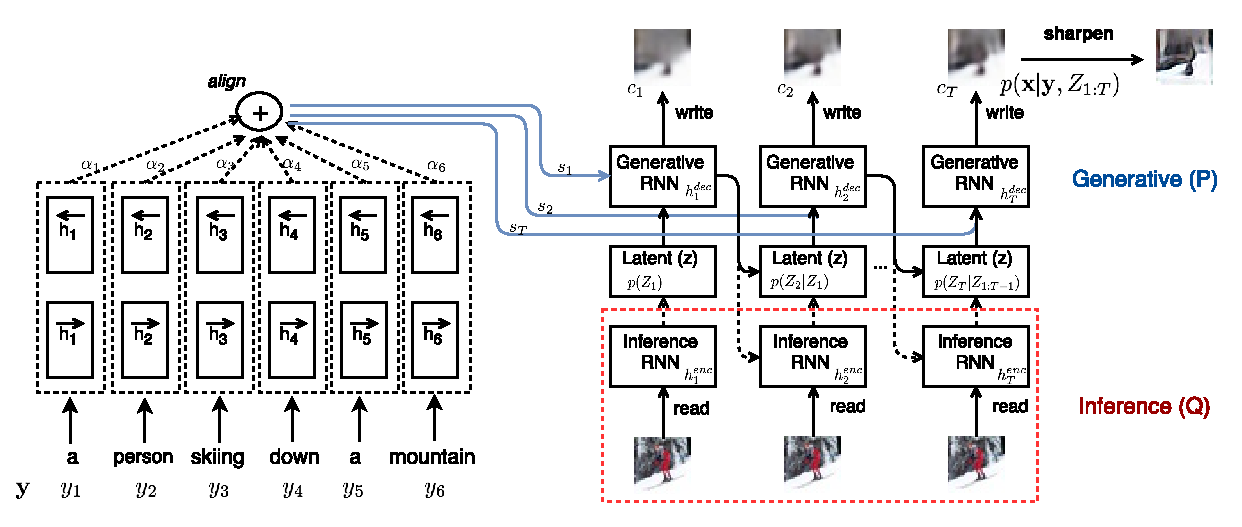
\includegraphics[width=0.99\textwidth]{figures/alignDrawAnnotated.pdf}\quad
%
\end{center}
\caption{The image of the proposed model}
\label{fig:figmodel}
\vspace{-0.3cm}
\end{figure}



\subsection{Image Model: the Conditional DRAW Network}

To generate images conditioned on the caption information, we extended the DRAW network \citep{gregor_draw} to include caption representation $\hlangall$ at each step, shown in Figure~\ref{fig:figmodel}. The conditional DRAW network is a stochastic recurrent neural network that consists of a set of latent variables $\Lat_t$ and accumulates the output at each iterative step..

Unlike the original DRAW network where latent variables are independent unit Gaussians $\mathcal{N}(0, I)$, the latent variables in the proposed alignDRAW model have their mean and variance depend on the previous recurrent hidden states $\hdec_{t-1}$ as in \cite{bachman_sdm}, except for $\lat_1 \sim \prior(\Lat_1) = \mathcal{N}(0, I)$. It has been shown in \citep{bachman_sdm} that model performance is improved by including dependencies between latent variables. Formally, the image is generated by iteratively computing the following equations for $t=1,...,T$ (see Figure~\ref{fig:figmodel}):
\begin{align}
\label{eq:x_hat}
\lat_t &\sim \prior(\Lat_t|\Lat_{1:t-1}) = \mathcal{N}(\mu_{t}(\hdec_{t-1}), \sigma_{t}(\hdec_{t-1})),\\
\hdec_t &= \decoder(\hdec_{t-1}, z_t, s_{t-1}), \\
s_{t} &= align(\hdec_{t-1}, \hlangall), \\
\canv_t &= \canv_{t-1} + \writeop(\hdec_t), 
\label{eq:write}
%\canv_t &= \canv_{t-1} + \writeop(\hdec_t)
\end{align}
where $\writeop$ and $\readop$ are the same attention operators as in \citep{gregor_draw}.
The $align$ function is used to compute the alignment between the input caption and intermediate image generative steps \citep{bahdanau_mt}. Given the caption representation from the language model, $\hlangall = [\hlang_{1}, \hlang_{2}, ..., \hlang_{N}]$, the $align$ operator outputs a dynamic sentence representation $s_t$ at each step through a weighted sum using alignment probabilities $\alpha_{1...N}$:
%\begin{align}
%\vspace{-0.1in}
$s_t=align(\hdec_{t-1}, \hlangall) = \alpha_{1}\hlang_{1} + \alpha_{2}\hlang_{2} + ... + \alpha_{N}\hlang_{N}.$
%\end{align}
The corresponding alignment probabilities $\alpha_{1...N}$ at each step are obtained using the caption representation $\hlangall$ and the hidden state of the generative model $\hdec_{t}$, as in \citep{bahdanau_mt}. The final canvas $\canv_T$ is transformed using a sigmoid function to produce an Bernoulli data likelihood over pixels given the latent variables and the input caption.


\comm{
We extended the architecture of the DRAW network to include an additional input caption from the language model described in Sec. (\ref{sec:lang}). Similarly to the original DRAW network, the conditional DRAW network is a stochastic recurrent neural network that consists of an Inference LSTM that infers the distribution of latent variables of image $x$ given caption $y$ and then a Generative LSTM that uses the inferred latent variables in order to reconstruct the image $x$ given caption $y$, where $\icaption$ is the input caption consisting of $N$ words $y_{1}, y_{2}, ..., y_{n}$. The $align$ function is used to compute the alignment between the input caption and intermediate image generative steps as in \cite{bahdanau_mt}:

Formally, the image is generated by iteratively computing the following equations for $t=1,...,T$
\begin{align}
\label{eq:x_hat}
\hat{x}_t &= x-\sigmoid(\canv_{t-1})\\
\label{eq:read}
r_t &= \readop(x_t, \hat{x}_t, \hdec_{t-1})\\
\henc_t &= \encoder(\henc_{t-1}, [r_t, \hdec_{t-1}])\\
\lat_t &\sim \post(\Lat_t|\henc_t)\\
\hdec_t &= \decoder(\hdec_{t-1}, z_t, s_{t-1})\\
s_{t} &= align(\hdec_{t-1}, \hlangall) \\
\label{eq:write}
\canv_t &= \canv_{t-1} + \writeop(\hdec_t)
\end{align}

where $\writeop$ is the same attention operators as in \citep{gregor_draw}.
%where $\readop$ and $\writeop$ are the same attention operators as in \citep{gregor_draw}.
% which apply a grid of Gaussian filters by specifying coordinates of the location and scale in order to yield a desirable image patch.
Given the caption representation from the language model, $\hlangall = [\hlang_{1}, \hlang_{2}, ..., \hlang_{N}]$, the $align$ operator computes the final sentence representation $s_t$ through a weighted sum using alignment probabilities $\alpha_{1...N}$:
\begin{align}
s_t=align(\hdec_{t-1}, \hlangall) = \alpha_{1}\hlang_{1} + \alpha_{2}\hlang_{2} + ... + \alpha_{N}\hlang_{N}.
\end{align}

The corresponding alignment probabilities $\alpha_{1...n}$ at each step are obtained by:
\begin{align}
e_{tj} &= v^{T}tanh(U\hlang_{j} + W\hdec_{t} + b)\\
\alpha_{j} &= \frac{exp(e_{tj})}{\sum_{j=1}^{N}exp(e_{tj})}.
\end{align}

Here $\hlang_{0}$ is initialized to the learned bias.
Setting $\alpha_{1...N}$ to $\frac{1}{N}$ turns the encoder into the vanilla model introduced in \citep{cho_mt} without the attention. 
}


\subsection{Learning}

%The model is learned by the modified version of Stochastic Gradient Variation Bayes (SGVB) algorithm introduced by \cite{kingma_vae}. 
The model is trained to maximize a variational lower bound $\loss$ on the marginal likelihood of the correct image $\oimage$ given the input caption $\icaption$, where $\loss = \sum_{\Lat}Q(\Lat\given\oimage,\icaption)\left(\log P(\oimage\given\icaption, \Lat_{1:T}) + \kldiv\left(Q(\Lat\given\oimage,\icaption)\klBars P(\Lat)\right)\right) \le \log P(\oimage\given\icaption)$ The posterior inference over the latent variables $\Lat_{1:T}$ is approximated using a inference recurrent neural net. Similarly to the DRAW network, the inference RNN produces an approximate posterior $Q(\Lat_{1:T}\given\oimage,\icaption)$ via a $\readop$ operator over the training image at each step. 
\begin{align}
\label{eq:x_hat}
\hat{\oimage}_t &= \oimage-\sigmoid(\canv_{t-1})\\
\label{eq:read}
r_t &= \readop(\oimage_t, \hat{\oimage}_t, \hdec_{t-1})\\
\henc_t &= \encoder(\henc_{t-1}, [r_t, \hdec_{t-1}])\\
\post(\Lat_t|\oimage,\icaption,\Lat_{1:t-1}) &= \mathcal{N}\left(\mu_t(\henc_t), \sigma_t(\henc_t)\right)
\end{align}

%The $\loss$ is decomposed into the latent loss $\lloss$ and the reconstruction loss $\rloss$. 

%The reconstruction loss $\rloss$ equals to $\frac{1}{L}\sum_{l=1}^{L}(log\,p(x_{t}|y,z)$ where $L$ is the number of samples used during training, which was set to $1$ in our experiments.

%The latent loss $\lloss$ is a negative sum of Kullback--Leibler divergence terms between distribution $\post(\Lat_t|\henc_t)$ and some prior distribution ${\prior(\Lat_t)}$ over time $t=1,...,T$, which can be seen as a regularization term. 
Since the prior distribution at time $t$ is dependent on the sufficient statistics of the prior distribution at time $t-1$. Namely, the mean and variance of $\prior(\Lat_t)$ depends on the $\hdec_{t-1}$. 
\begin{align}
\mu_{t}^{prior} &= tanh(W_{\mu}\hdec_{t-1})\\
\sigma_{t}^{prior} &= exp(tanh(W_{\sigma}\hdec_{t-1})) 
\end{align}

The terms in the variational lower bound are rearranged using the law of total expectation. Therefore, the loss function $\loss$ is calculated as follows:
\begin{align}
\loss =  &\expectation_{Q(\Lat_{1:t}\given\icaption,\oimage)}\left[ - \log p(\oimage\given\icaption,\Lat_{1:T}) + \sum_{t=2}^T\kldiv\left(\post(\Lat_t\given\Lat_{t-1},\icaption,\oimage)\klBars\prior(\Lat_t\given\Lat_{t-1},\icaption)\right) \right] \nonumber \\& + \kldiv\left(\post(\Lat_1\given\icaption,\oimage)\klBars\prior(\Lat_1\given\icaption)\right).
\end{align}
The expectation can be approximate by $\numSamples$ Monte Carlo samples $\LatSample_{1:T}$ from $\post(\Lat_{1:T}\given\icaption, \oimage)$:
\begin{align}
\loss \approx  &\frac{1}{\numSamples}\sum_{\sampleIdx=1}^\numSamples\left[ - \log p(\oimage\given\icaption,\LatSample^\sampleIdx_{1:T}) + \sum_{t=2}^T\kldiv\left(\post(\Lat_t\given\LatSample^\sampleIdx_{t-1},\icaption,\oimage)\klBars\prior(\Lat_t\given\LatSample^\sampleIdx_{t-1},\icaption)\right) \right] \nonumber \\& + \kldiv\left(\post(\Lat_1\given\icaption,\oimage)\klBars\prior(\Lat_1\given\icaption)\right).
\end{align}
\comm{
\begin{align}
\loss &= -\sum_{t=1}^{T}D_{KL}(\post(\Lat_t|\henc_t,s_{t-1})\,||\,\prior(\Lat_t)) + \frac{1}{L}\sum_{l=1}^{L}log\,p(x_{t}|y,z)\\
&=
\frac{1}{2}\sum_{t=1}^{T}(1 - 2\,log\,\sigma_{t}^{prior} + 2\,log\,\sigma_{t} - \frac{exp(2\,log\,\sigma_{t}) + (\mu_{t} - \mu_{t}^{prior})^{2}}{exp(2\,log\,\sigma_{t}^{prior})}) + \frac{1}{L}\sum_{l=1}^{L}log\,p(x_{t}|y,z)
\end{align}
}

\subsection{Generating Images from Captions}

During the image generation step, we discard the inference network and instead sample from the prior distribution. 
Due to the blurriness of samples generated by the DRAW model, we perform an additional post processing step where we use a 
adversarial network trained on residuals of a laplacian pyramid 
to sharpen the generated images, similar to \citep{denton_lapgan}. By fixing the prior of the adversarial generator to its mean, it gets treated as a deterministic neural network which allows us to calculate the lower bound of likelihood. The reconstuction loss becomes the loss between sharpened image and correct image, whereas the latent loss stays the same. Additionally, we noticed that sampling from the mean of uniform distribution generated samples with less noise than if we had otherwise sampled from the uniform distribution itself.  

\section{Experiments}
\subsection{MNIST With Captions}
As a first experiment, we trained our proposed model on the MNIST dataset with artificial captions. Either one or two digits from the MNIST training dataset were placed on a $60 \times 60$ blank image. One digit was placed in one of the four (top-left, top-right, bottom-left or bottom-right) corners of the image. Two digits were either placed horizontally or vertically in nonoverlapping fashion. 
While many generative models are trained on the binarized version of the MNIST dataset, we trained directly on pixel intensities with a binary cross entropy cost function. 
The generated images and the attention alignment are displayed in Figure~\ref{fig:figmnist}.

\begin{figure}[!t]
\captionsetup[subfigure]{labelformat=empty}
\begin{center}
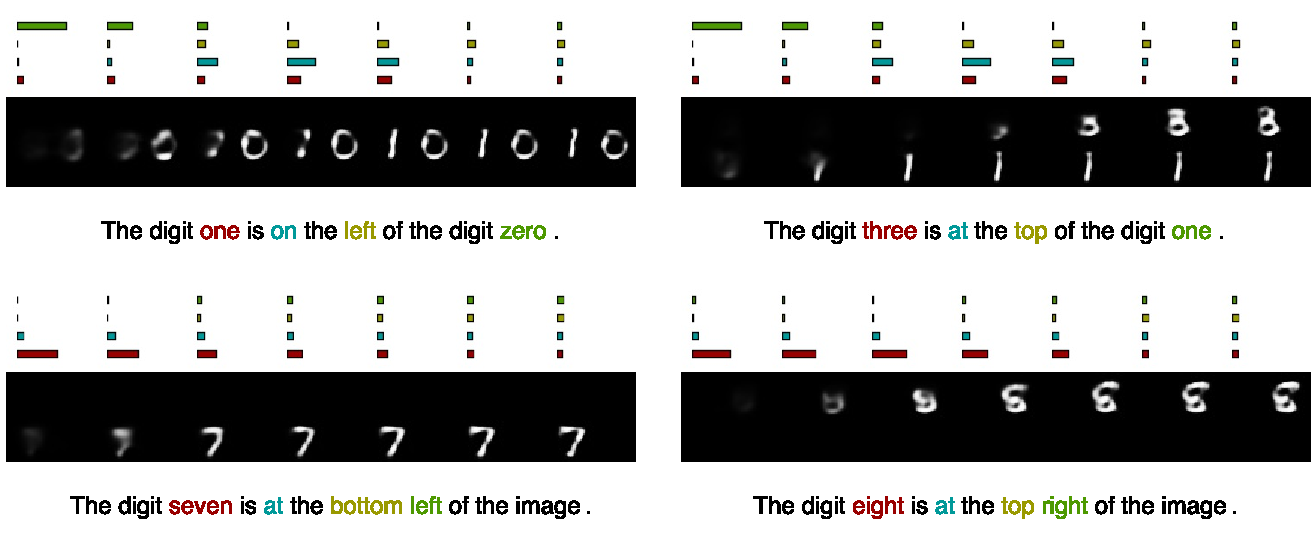
\includegraphics[width=0.99\textwidth]{figures/new/mnist/test3.pdf}\quad
%
\end{center}
\caption{Examples of generating $60 \times 60$ images corresponding to respective captions. Examples at the \textbf{left column} were present during training, whereas the \textbf{right column} examples were hidden during training.}
\label{fig:figmnist}
\vspace{-0.3cm}
\end{figure}

\subsection{Microsoft COCO}

Microsoft COCO \citep{mscoco} is a very large dataset of roughly 83k images, each annotated with 5 captions. The rich collection of images with a wide variety of styles, backgrounds and objects makes the task of learning a good generative model 
%conditioned on a caption 
very challenging. For consistency with related work on caption generation, we use only five captions when training our model. In the following subsections, we analyze both the qualitative and quantitative aspects of our model as well as compare its performance with that of other, related generative models.

\subsubsection{Analysis of Generated Images}
The main goal of this work is to learn a model that can understand the semantic meaning expressed in the textual descriptions of images, such as the properties of objects, the relationships between them, etc. and then use that knowledge to generate relevant images. To examine the understanding of our model, we wrote a set of captions inspired by the COCO dataset and changed some words in the captions to see whether the model made the relevant changes in the generated samples.

First, we wanted to see whether the model understood one of the most basic properties of any object, the color. In Figure~\ref{fig:genimages1}, we generated images of school buses with four different colors: yellow, red, green and blue. Although, there are images of buses with different colors in the training set, all mentioned school buses are specifically colored yellow. Despite that, the model managed to generate images of an object that is visually reminiscent of a school bus that is painted with the specified color.

\begin{figure}[!h]
\captionsetup[subfigure]{labelformat=empty}
\begin{center}
\subfloat[A \underline{yellow} school bus parked in a parking lot.
]{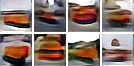
\includegraphics[width=0.23\textwidth]{figures/new/a-yellow-school-bus-parked-in-a-parking-lot-sharp.png}}\quad
%
\subfloat[A \underline{red} school bus parked in a parking lot.
]{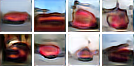
\includegraphics[width=0.23\textwidth]{figures/new/a-red-school-bus-parked-in-a-parking-lot-sharp.png}}\quad
%
\subfloat[A \underline{green} school bus parked in a parking lot.
]{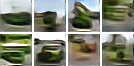
\includegraphics[width=0.23\textwidth]{figures/new/a-green-school-bus-parked-in-a-parking-lot-sharp.png}}\quad
%
\subfloat[A \underline{blue} school bus parked in a parking lot.
]{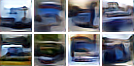
\includegraphics[width=0.23\textwidth]{figures/new/a-blue-school-bus-parked-in-a-parking-lot-sharp.png}}\quad
%
\end{center}
\caption{Examples of changing the color while keeping the caption fixed.}
\label{fig:genimages1}
\vspace{-0.3cm}
\end{figure}

Apart from changing the colors of objects, we were curious whether changing the background of the scene described in a caption would result in the appropriate changes in the generated samples. The task of changing the background of an image is somewhat harder than just changing the color of an object because the model will have to make alterations over a wider visual area. Nevertheless, as shown in Figure~\ref{fig:genimages2} changing the skies from blue to rainy in a caption as well as changing the grass type from dry to green in another caption resulted in the appropriate changes in the generated image. The nearest images from the training set also indicate that the model was not simply copying the patterns it observed during the learning phase.

\begin{figure}[!h]
\captionsetup[subfigure]{labelformat=empty}
\begin{center}
\subfloat[]{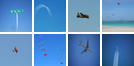
\includegraphics[width=0.23\textwidth]{figures/new/a-very-large-commercial-plane-flying-in-blue-skies-closest.png}}\quad
%
\subfloat[]{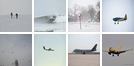
\includegraphics[width=0.23\textwidth]{figures/new/a-very-large-commercial-plane-flying-in-rainy-skies-closest.png}}\quad
%
\subfloat[]{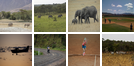
\includegraphics[width=0.23\textwidth]{figures/new/a-herd-of-elephants-walking-across-a-dry-grass-field-closest.png}}\quad
%
\subfloat[]{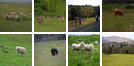
\includegraphics[width=0.23\textwidth]{figures/new/a-herd-of-elephants-walking-across-a-green-grass-field-closest.png}}\\
\vspace{-0.45cm}
%
\subfloat[A very large commercial plane flying in \underline{blue} skies.
]{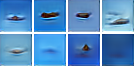
\includegraphics[width=0.23\textwidth]{figures/new/a-very-large-commercial-plane-flying-in-blue-skies-sharp.png}}\quad
%
\subfloat[A very large commercial plane flying in \underline{rainy} skies.
]{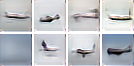
\includegraphics[width=0.23\textwidth]{figures/new/a-very-large-commercial-plane-flying-in-rainy-skies-sharp.png}}\quad
%
\subfloat[A herd of elephants walking across a \underline{dry} grass field.
]{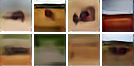
\includegraphics[width=0.23\textwidth]{figures/new/a-herd-of-elephants-walking-across-a-dry-grass-field-sharp.png}}\quad
%
\subfloat[A herd of elephants walking across a \underline{green} grass field.
]{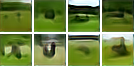
\includegraphics[width=0.23\textwidth]{figures/new/a-herd-of-elephants-walking-across-a-green-grass-field-sharp.png}}\quad
%
\end{center}
\caption{\textbf{Bottom}: Examples of changing the background while keeping the caption fixed. \textbf{Top}: The respective nearest training images based on pixel-wise L2 distance.}
\label{fig:genimages2}
\vspace{-0.3cm}
\end{figure}

Despite a large number of ways of changing colors and backgrounds in descriptions, in general we found that the model made appropriate changes as long as some similar pattern was present in the training set. However, the model struggled when the visual difference between objects was very small, such as when the objects have the same general shape and color. In Figure~\ref{fig:genimages3}, we demonstrate that when we swap two objects that are both visually similar, for example cats and dogs, it is difficult to discriminate solely from the generated samples whether it is an image of a cat or dog, even though we might notice an animal-like shape. This highlights a limitation of the model in that it has difficulty modelling the fine-grained details of objects. 
 
\begin{figure}[!h]
\captionsetup[subfigure]{labelformat=empty}
\begin{center}
\subfloat[\underline{The decadent chocolate} \underline{desert} is on the table.
]{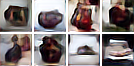
\includegraphics[width=0.23\textwidth]{figures/new/the-decadent-chocolate-dessert-is-on-the-table-sharp.png}}\quad
%
\subfloat[\underline{A bowl of bananas} is on the table.
]{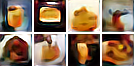
\includegraphics[width=0.23\textwidth]{figures/new/a-bowl-of-bananas-is-on-the-table-sharp.png}}\quad
%
\subfloat[A vintage photo of a \underline{cat}.
]{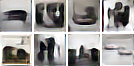
\includegraphics[width=0.23\textwidth]{figures/new/a-vintage-photo-of-a-cat-sharp.png}}\quad
%
\subfloat[A vintage photo of a \underline{dog}.
]{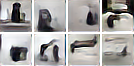
\includegraphics[width=0.23\textwidth]{figures/new/a-vintage-photo-of-a-dog-sharp.png}}\quad
%
\end{center}
\caption{Examples of changing the object while keeping the caption fixed.}
\label{fig:genimages3}
\vspace{-0.3cm}
\end{figure}

As a test of model generalization, we tried generating images corresponding to captions that describe scenarios that are highly unlikely to occur in real life. These captions describe some common object doing unusual things 
or in a strange location.
%that are impossible in the real world. 
%considering the physics of real world. 
Even though these scenarios may never happen in real life, it is very easy for humans to imagine the corresponding scene. Nevertheless, as you can see in Figure~\ref{fig:genimages4}, the model managed to generate reasonable images.  

\begin{figure}[!h]
\captionsetup[subfigure]{labelformat=empty}
\begin{center}
\subfloat[A stop sign is flying in blue skies.
]{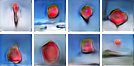
\includegraphics[width=0.23\textwidth]{figures/new/a-stop-sign-is-flying-in-blue-skies-sharp.png}}\quad
%
\subfloat[A herd of elephants flying in the blue skies.
]{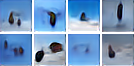
\includegraphics[width=0.23\textwidth]{figures/new/a-herd-of-elephants-flying-in-the-blue-skies-sharp.png}}\quad
%
\subfloat[A toilet seat sits open in the grass field.
]{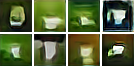
\includegraphics[width=0.23\textwidth]{figures/new/a-toilet-seat-sits-open-in-the-grass-field-sharp.png}}\quad
%
\subfloat[A person skiing on sand clad vast desert.
]{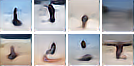
\includegraphics[width=0.23\textwidth]{figures/new/a-person-skiing-on-sand-clad-vast-desert-sharp.png}}\quad
%
\end{center}
\caption{Examples of novel scene compositions.}
\label{fig:genimages4}
\vspace{-0.3cm}
\end{figure}

\subsubsection{Analysis of Attention}

After flipping sets of words in the captions, we were curious to see which words the model attended to when generating images. It turned out that during the generation step, the model mostly focused on the specific words (or their neighbors) that carried the main semantic meaning expressed in the sentences. The attention values in sentences helped us interpret the reasons why the model made the changes it did when we flipped certain words. For example, in Figure~\ref{fig:attentimages1} we can see that when we flipped the word ``desert'' to ``forest'', the attention over words in the sentence did not change drastically. This suggests that, in their respective sentences, the model looked at ``desert'' and ``forest'' with relatively equal probability, and thus made the correct changes. In contrast, when we swap words ``beach'' and ``sun'', we can see a drastic change between sentences in the probability distribution over words. By noting that the model completely ignores the word ``sun'' in the second sentence, we can therefore gain a more thorough understanding of why we see no visual differences between the images generated by each caption.

We also tried to analyze the way the model generated images. Unfortunately, we found that there was no significant connection between the patches drawn on canvas and the most attended words at particular timesteps.

\begin{figure}[!h]
\captionsetup[subfigure]{labelformat=empty}
\begin{center}
\subfloat[\hlcthree{A} rider \hlcone{on} a blue \hlcone{motorcycle} in the \underline{\hlctwo{desert}}.
]{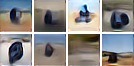
\includegraphics[width=0.23\textwidth]{figures/new/a-rider-on-a-blue-motorcycle-in-the-desert-sharp.png}}\quad
%
\subfloat[\hlcthree{A} rider \hlcone{on} a blue \hlcone{motorcycle} in the \underline{\hlctwo{forest}}.
]{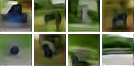
\includegraphics[width=0.23\textwidth]{figures/new/a-rider-on-a-blue-motorcycle-in-the-forest-sharp.png}}\quad
%
\subfloat[\hlctwo{A} \hlcone{surfer}, a woman, and a child walk on the \underline{\hlctwo{beach}}.
]{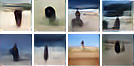
\includegraphics[width=0.23\textwidth]{figures/new/a-surfer-,-a-woman-,-and-a-child-walk-on-the-beach-sharp.png}}\quad
%
\subfloat[\hlcthree{A} \hlcone{surfer}, a woman, and a child walk on the \underline{\hlczero{sun}}.
]{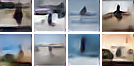
\includegraphics[width=0.23\textwidth]{figures/new/a-surfer-,-a-woman-,-and-a-child-walk-on-the-sun-sharp.png}}\quad
%
\end{center}
\caption{Examples of most attended words while changing the background in the caption.}
\label{fig:attentimages1}
\vspace{-0.3cm}
\end{figure} 

\subsubsection{Comparison With Other Models}
Quantitatively evaluating generative models remains a challenging task in of itself as each method of evaluation suffers from its own specific drawbacks. Compared to reporting classification accuracies in discriminative models, the measures defining generative models are intractable most of the times and might not correctly define the real quality of the model. To get a better comparison between performances of different generative models, we report results on two different metrics as well as a qualitative comparison of different generative models.

\begin{figure}[!t]
\captionsetup[subfigure]{labelformat=empty}
\begin{center}
\subfloat[Align DRAW]{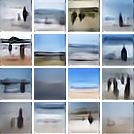
\includegraphics[width=0.23\textwidth]{figures/new/a-group-of-people-walk-on-a-beach-with-surf-boards-sharp.png}}\quad
%
\subfloat[LAPGAN]{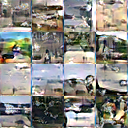
\includegraphics[width=0.23\textwidth]{figures/a-group-of-people-walk-on-a-beach-with-surf-boards-lapgan.png}}\quad
%
\subfloat[Conv. VAE]{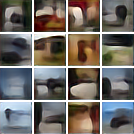
\includegraphics[width=0.23\textwidth]{figures/a-group-of-people-walk-on-a-beach-with-surf-boards-convdeconvvae.png}}\quad
%
\subfloat[Fully-conn. VAE]{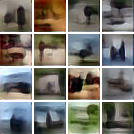
\includegraphics[width=0.23\textwidth]{figures/a-group-of-people-walk-on-a-beach-with-surf-boards-fcvae.png}}\quad
%
\end{center}
\caption{Four different models displaying results from sampling caption \textit{A group of people walk on a beach with surf boards.}}
\label{fig:diffmodels}
\vspace{-0.2cm}
\end{figure}

We compared the performance of the proposed model to the DRAW model conditioned on captions without align function (noalignDRAW) as well as the DRAW model conditioned on skipthought vectors (skipthoughtDRAW). All of the conditional DRAW models were trained with binary cross entropy cost function. We also compared our model with Fully-connected (FC) and Convolutional-Deconvolutional (Conv.) Variational Autoencoders which were trained with the least squares cost function. The LAPGAN model was trained on two level Laplacian Pyramid and was conditioned on the skipthought vectors. 

In Figure~\ref{fig:diffmodels}, we generated several samples from the prior of each of the current state-of-the-art generative models, conditioned on the caption ``A group of people walk on a beach with surf boards". While all of the samples look sharp, the images generated by LAPGAN look more noisy and it is harder to make out definite objects, whereas the images generated by variational models trained with L2 cost function have a watercolor effect on the images.

As for the quantitative comparison of different models, we first compare the performances of the model trained with variational methods. We rank the images in the test set conditioned on the captions based on the the variational lower bound of likelihood and then report the Precision-Recall metric as an evaluation of the quality of the generative model (see Table~\ref{tab:results}.). Unsurprisingly, the quality of image retrieval using generative models is worse than that of discriminative models that were specifically built for retrieval. To deal with the large computational complexity involved in looping through each test image, we create a shortlist of one hundred images including the correct one, based on the images having the closest distance in the convolutional feature-space of a VGG-like model trained on the CIFAR dataset. Since there are ``easy'' images for which the model assigns high likelihood independent of the query caption, we look at the ratio of likelihood of image conditioned on the sentence to likelihood of image conditioned on the mean sentence representation in the training set \cite{kiros_captions}. We found that the reconstruction error $\rloss$ increased for sharpened images, and that sharpening considerably hurt the retrieval results. Since sharpening changes the statistics of images, computing reconstruction error for each pixel is not necessarily a good metric.

Instead of calculating error per pixel, we turn to a smarter metric, the Structural Similarity Index (SSI), which incorporates luminance and contrast masking into the error calculation. Due to strong inter-dependencies of closer pixels, the metric is calculated on small windows of the image. Due to independence property of test captions, we sampled fifty images from the prior of each generative model for every caption in the test set in order to calculate SSI. The results are reported in Table~\ref{tab:results}.

\begin{table}[!b]
\begin{center}
\begin{tabulary}{\linewidth}{c || c c c c c || c}
\hline
\multicolumn{7}{c}{\textbf{COCO (before sharpening)}} \\
\hline
& \multicolumn{5}{c||}{Image Search} & Image Similarity \\
%\cline{2-6}
\textbf{Model} & \textbf{R@1} & \textbf{R@5} & \textbf{R@10} & \textbf{R@50} & \textbf{Med r} & \textbf{SSI} \\
\hline
\hline
LAPGAN & - & - & - & - & - & 0.08 \\ % - & - & - & - & - & 0.08
\hline
Fully-conn. VAE (L2 cost) & 1.0 & 5.6 & 10.4 & 51.1 & 51 & 0.156 \\ % 0.688 & 4.58 & 8.74 & 46.832 & 54 & -1
Conv. VAE (L2 cost) & 1.0 & 5.9 & 10.9 & 50.8 & 50 & \textbf{0.164} \\ % 0.672 & 4.448 & 8.476 & 46.596 & 54 & 0.131
Skipthought DRAW & 2.6 & 12.6 & 21.3 & 66.9 & 33 & 0.157 \\ % 0.988 & 6.18 & 11.48 & 52.512 & 48 & 0.118
Noalign DRAW & 3.2 & \textbf{16.3} & \textbf{26.0} & 72.5 & \textbf{27} & 0.155 \\ % 1.0 & 6.124 & 11.18 & 52.112 & 48 & 0.114
Align DRAW & \textbf{3.6} & 16.1 & \textbf{26.0} & \textbf{72.8} & 28 & 0.156 \\ % 0.924 & 6.216 & 11.184 & 52.492 & 48 & 0.115
\end{tabulary}
\end{center}
\end{table}

% \begin{table}[!t]
% \begin{center}
% \begin{tabulary}{\linewidth}{c || c c c c c || c}
% \hline
% \multicolumn{7}{c}{\textbf{COCO (before sharpening)}} \\
% \hline
% & \multicolumn{5}{c||}{Image Search} & Image Similarity \\
% %\cline{2-6}
% \textbf{Model} & \textbf{R@1} & \textbf{R@5} & \textbf{R@10} & \textbf{R@50} & \textbf{Med r} & \textbf{SSI} \\
% \hline
% \hline
% LAPGAN & - & - & - & - & - & 0.08 \\ % - & - & - & - & - & 0.08
% \hline
% Fully-conn. VAE (L2 cost) & 0.7 & 4.6 & 8.7 & 46.8 & 54 & 0.122 \\ % 0.688 & 4.58 & 8.74 & 46.832 & 54 & -1
% Conv. VAE (L2 cost) & 0.7 & 4.4 & 8.5 & 46.6 & 54 & \textbf{0.131} \\ % 0.672 & 4.448 & 8.476 & 46.596 & 54 & 0.131
% Noalign DRAW & \textbf{1.0} & 6.1 & 11.2 & 52.1 & \textbf{48} & 0.114 \\ % 1.0 & 6.124 & 11.18 & 52.112 & 48 & 0.114
% Skipthought DRAW & \textbf{1.0} & \textbf{6.2} & \textbf{11.5} & \textbf{52.5} & \textbf{48} & 0.118 \\ % 0.988 & 6.18 & 11.48 & 52.512 & 48 & 0.118
% Align DRAW & 0.9 & \textbf{6.2} & 11.2 & \textbf{52.5} & \textbf{48} & 0.115 \\ % 0.924 & 6.216 & 11.184 & 52.492 & 48 & 0.115
% \end{tabulary}
% \end{center}
% \end{table}

\section{Discussion}

We have shown that our proposed model manages to generate reasonable images corresponding to respective captions as well as generalize to completely novel scenarios that never occur in real life. Sequential generation of images using attention played a crutial part in it. However the DRAW model still underfits on training data which leads to the blurry samples. We think that extending this process by generating very small sections of images like superpixels over potentially hundreds of timesteps might help the model fit the data and generate sharp images.

\section{Acknowledgements}
We would like to thank developers of Theano for a powerful software and authors of \cite{denton_lapgan} for open sourcing their code. We would also like to thank Ryan Kiros and Nitish Srivastava for helpful discussions. We will release our code with pretrained models as soon as we clean it. Acknowledging funding (Russ)

\bibliography{iclr-paper}
\bibliographystyle{iclr-style/iclr2016_conference}

\newpage
\appendix


\section*{Appendix A: MNIST With Captions}

\begin{figure}[!t]
\captionsetup[subfigure]{labelformat=empty}
\begin{center}
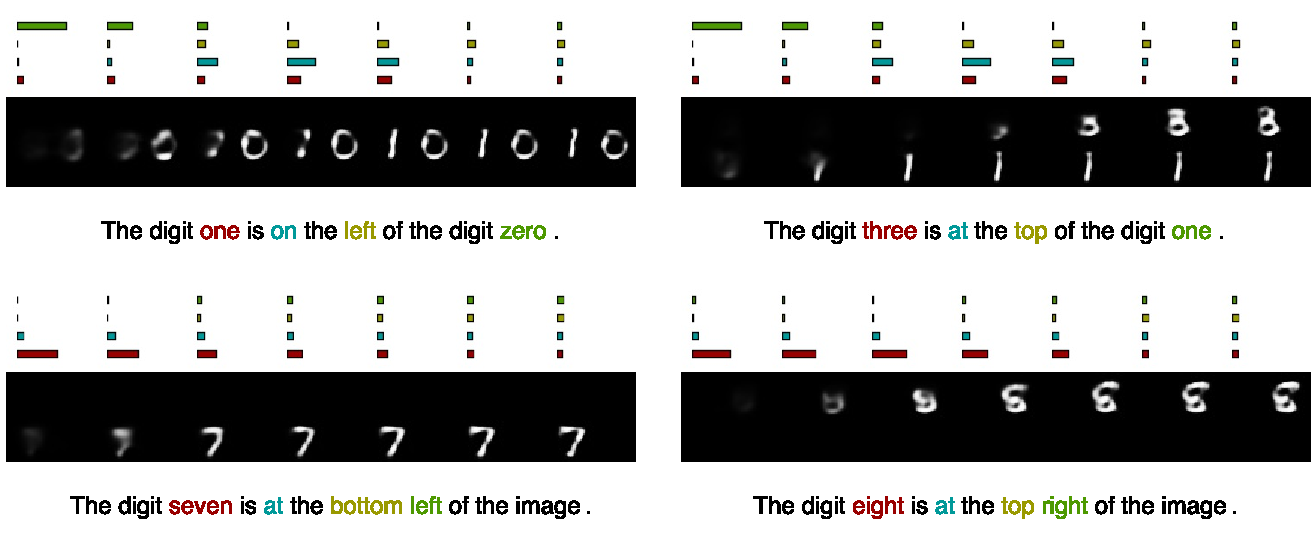
\includegraphics[width=0.99\textwidth]{figures/new/mnist/test3.pdf}\quad
%
\end{center}
\caption{Examples of generating $60 \times 60$ MNIST images corresponding to respective captions. The captions on the \textbf{left column} were part of the training set. The digits described in the captions on the \textbf{right column} were hidden during training for the respective configurations.}
\label{fig:figmnist}
\vspace{-0.3cm}
\end{figure}

As an additional experiment, we trained our model on the MNIST dataset with artificial captions. Either one or two digits from the MNIST training dataset were placed on a $60 \times 60$ blank image. One digit was placed in one of the four (top-left, top-right, bottom-left or bottom-right) corners of the image. Two digits were either placed horizontally or vertically in nonoverlapping fashion. The corresponding artificial captions specified the 
identity of each digit along with their relative positions, e.g. ``The digit two is on the top  
of the digit zero'', or ``The digit seven is at the bottom left of the image''.  

The generated images together with the attention alignments are displayed in Figure~\ref{fig:figmnist}. The model correctly displayed the specified digits at the described positions and even managed to generalize 
reasonably well to the configurations that were never present during training.
In the case of generating two digits, the model would dynamically attend 
to the digit in the caption it was drawing at that particular time-step. 
Similarly, in the setting where the caption specified only a single digit, the model would correctly 
attend to the digit in the caption during the whole generation process. 
In both cases, the model placed small attention values on the words describing the position of digits in the images.

\section*{Appendix B: Training Details}
\label{sec:training_details}

\subsection*{Hyperparameters}

Each parameter in alignDRAW was initialized by sampling from a Gaussian distribution with 
mean $0$ and standard deviation $0.01$. The model was trained using \textit{RMSprop} with an initial learning rate of $0.001$. The norm of the gradients was clipped at a maximum of $10.0$ during training to deal with exploding gradients. We used a vocabulary size of $K = 25323$ and $K = 22$ for Microsoft COCO and MNIST with Captions respectively. All capital letters in the words were converted to small letters as a preprocessing step. For all tasks, $\overrightarrow{h}^{lang}_{n}$ and $\overleftarrow{h}^{lang}_{n}$ in the language model had $128$ units. The parameters in the \textit{align} operator had a dimensionality of $l = 512$, $\vv \in \mathbb{R}^{512}$, $U \in \mathbb{R}^{512 \times 128}$, $W \in \mathbb{R}^{512 \times n^{gen}}$ and $b \in \mathbb{R}^{512}$. For the Microsoft COCO task, the alignDRAW model was trained for $18$ epochs and the learning rate was reduced by the factor of $0.1$ after $11$ epochs. The architectural configurations of alignDRAW models are shown on Table~\ref{tab:drawhyper}.

\begin{table}[!t]
\begin{center}
\begin{tabulary}{\linewidth}{c | c c c c c c}
\hline
\multicolumn{7}{c}{\textbf{alignDRAW Model}} \\
\hline
Task & \#glimpses & Inference \#$h$ & Generative \#$h$ & \#$z$ & Read Size & Write Size\\
\hline
Microsoft COCO & 32 & 550 & 550 & 275 & 9 & 9\\
MNIST Captions & 32 & 300 & 300 & 150 & 8 & 8\\
\end{tabulary}
\caption{The architectural configurations of alignDRAW models.}
\label{tab:drawhyper}
\end{center}
%\vspace{-0.3cm}
\end{table}

The GAN model used for sharpening had the same configuration as the $28 \times 28$ model trained by \cite{denton_lapgan} on the edge residuals of the CIFAR dataset. The configuration can be found at \url{https://gist.github.com/soumith/e3f722173ea16c1ea0d9}. The model was trained for $6$ epochs. 
For the LAPGAN model, we used a data augmentation step where we took 5 crops (top-left, top-right, bottom-left, bottom-right, center) of a downsampled COCO image and assigned each crop one of the 5 captions that described the uncropped image.

\subsection*{Evaluation}

Table~\ref{tab:nll} shows the estimated variational lower bound on the average train/validation/test 
log-probabilities.
Note that the alignDRAW model does not suffer much from overfitting. 
The results worsened dramatically after sharpening test images.

\begin{table}[!h]
\begin{center}
\begin{tabulary}{\linewidth}{c | c c c c}
\hline
Model & Train LL & Valid LL & Test LL & Test LL (after sharpening)\\
\hline
skipthoughtDRAW & -1794.29 & -1797.41 & -1791.37 & -2045.84 \\
noalignDRAW & -1792.14 & -1796.94 & -1791.15 & -2051.07 \\
alignDRAW & -1792.15 & -1797.24 & -1791.53 & -2042.31
\end{tabulary}
\caption{The lower bound on the average test log-probabilities of conditional DRAW models, trained on the Microsoft COCO dataset.}
\label{tab:nll}
\end{center}
\end{table}

\newpage
\section*{Appendix C: Effect of Sharpening Images.}
\label{sec:post_processing}

\begin{figure}[!h]
\captionsetup[subfigure]{labelformat=empty}
\vspace{-0.27in}
\begin{center}
\subfloat[]{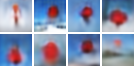
\includegraphics[width=0.23\textwidth]{figures/new/a-stop-sign-is-flying-in-blue-skies-blurry.png}}\quad
%
\subfloat[]{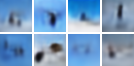
\includegraphics[width=0.23\textwidth]{figures/new/a-herd-of-elephants-flying-in-the-blue-skies-blurry.png}}\quad
%
\subfloat[]{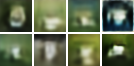
\includegraphics[width=0.23\textwidth]{figures/new/a-toilet-seat-sits-open-in-the-grass-field-blurry.png}}\quad
%
\subfloat[]{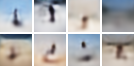
\includegraphics[width=0.23\textwidth]{figures/new/a-person-skiing-on-sand-clad-vast-desert-blurry.png}}\\
\vspace{-0.45cm}
%
\subfloat[%A stop sign is flying in blue skies.
]{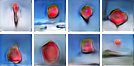
\includegraphics[width=0.23\textwidth]{figures/new/a-stop-sign-is-flying-in-blue-skies-sharp.png}}\quad
%
\subfloat[%A herd of elephants flying in the blue skies.
]{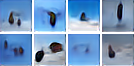
\includegraphics[width=0.23\textwidth]{figures/new/a-herd-of-elephants-flying-in-the-blue-skies-sharp.png}}\quad
%
\subfloat[%A toilet seat sits open in the grass field.
]{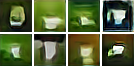
\includegraphics[width=0.23\textwidth]{figures/new/a-toilet-seat-sits-open-in-the-grass-field-sharp.png}}\quad
%
\subfloat[%A person skiing on sand clad vast desert.
]{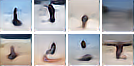
\includegraphics[width=0.23\textwidth]{figures/new/a-person-skiing-on-sand-clad-vast-desert-sharp.png}}\\
%

\subfloat[]{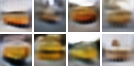
\includegraphics[width=0.23\textwidth]{figures/new/a-yellow-school-bus-parked-in-a-parking-lot-blurry.png}}\quad
%
\subfloat[]{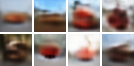
\includegraphics[width=0.23\textwidth]{figures/new/a-red-school-bus-parked-in-a-parking-lot-blurry.png}}\quad
%
\subfloat[]{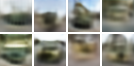
\includegraphics[width=0.23\textwidth]{figures/new/a-green-school-bus-parked-in-a-parking-lot-blurry.png}}\quad
%
\subfloat[]{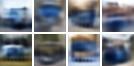
\includegraphics[width=0.23\textwidth]{figures/new/a-blue-school-bus-parked-in-a-parking-lot-blurry.png}}\\
\vspace{-0.45cm}
%
\subfloat[%A yellow school bus parked in a parking lot.
]{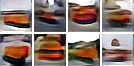
\includegraphics[width=0.23\textwidth]{figures/new/a-yellow-school-bus-parked-in-a-parking-lot-sharp.png}}\quad
%
\subfloat[%A red school bus parked in a parking lot.
]{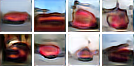
\includegraphics[width=0.23\textwidth]{figures/new/a-red-school-bus-parked-in-a-parking-lot-sharp.png}}\quad
%
\subfloat[%A green school bus parked in a parking lot.
]{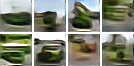
\includegraphics[width=0.23\textwidth]{figures/new/a-green-school-bus-parked-in-a-parking-lot-sharp.png}}\quad
%
\subfloat[%A blue school bus parked in a parking lot.
]{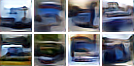
\includegraphics[width=0.23\textwidth]{figures/new/a-blue-school-bus-parked-in-a-parking-lot-sharp.png}}\\
%

\subfloat[]{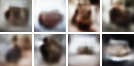
\includegraphics[width=0.23\textwidth]{figures/new/the-decadent-chocolate-dessert-is-on-the-table-blurry.png}}\quad
%
\subfloat[]{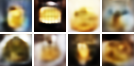
\includegraphics[width=0.23\textwidth]{figures/new/a-bowl-of-bananas-is-on-the-table-blurry.png}}\quad
%
\subfloat[]{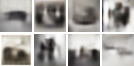
\includegraphics[width=0.23\textwidth]{figures/new/a-vintage-photo-of-a-cat-blurry.png}}\quad
%
\subfloat[]{\includegraphics[width=0.23\textwidth]{figures/new/a-vintage-photo-of-a-dog-blurry.png}}\\
\vspace{-0.45cm}
%
\subfloat[%The decadent chocolate desert is on the table.
]{\includegraphics[width=0.23\textwidth]{figures/new/the-decadent-chocolate-dessert-is-on-the-table-sharp.png}}\quad
%
\subfloat[%A bowl of bananas is on the table.
]{\includegraphics[width=0.23\textwidth]{figures/new/a-bowl-of-bananas-is-on-the-table-sharp.png}}\quad
%
\subfloat[%A vintage photo of a cat.
]{\includegraphics[width=0.23\textwidth]{figures/new/a-vintage-photo-of-a-cat-sharp.png}}\quad
%
\subfloat[%A vintage photo of a dog.
]{\includegraphics[width=0.23\textwidth]{figures/new/a-vintage-photo-of-a-dog-sharp.png}}\\
%

\subfloat[]{\includegraphics[width=0.23\textwidth]{figures/new/a-very-large-commercial-plane-flying-in-blue-skies-blurry.png}}\quad
%
\subfloat[]{\includegraphics[width=0.23\textwidth]{figures/new/a-very-large-commercial-plane-flying-in-rainy-skies-blurry.png}}\quad
%
\subfloat[]{\includegraphics[width=0.23\textwidth]{figures/new/a-herd-of-elephants-walking-across-a-dry-grass-field-blurry.png}}\quad
%
\subfloat[]{\includegraphics[width=0.23\textwidth]{figures/new/a-herd-of-elephants-walking-across-a-green-grass-field-blurry.png}}\\
\vspace{-0.45cm}
%
\subfloat[%A very large commercial plane flying in blue skies.
]{\includegraphics[width=0.23\textwidth]{figures/new/a-very-large-commercial-plane-flying-in-blue-skies-sharp.png}}\quad
%
\subfloat[%A very large commercial plane flying in rainy skies.
]{\includegraphics[width=0.23\textwidth]{figures/new/a-very-large-commercial-plane-flying-in-rainy-skies-sharp.png}}\quad
%
\subfloat[%A herd of elephants walking across a dry grass field.
]{\includegraphics[width=0.23\textwidth]{figures/new/a-herd-of-elephants-walking-across-a-dry-grass-field-sharp.png}}\quad
%
\subfloat[%A herd of elephants walking across a green grass field.
]{\includegraphics[width=0.23\textwidth]{figures/new/a-herd-of-elephants-walking-across-a-green-grass-field-sharp.png}}\\
%

\subfloat[]{\includegraphics[width=0.23\textwidth]{figures/new/a-rider-on-a-blue-motorcycle-in-the-desert-blurry.png}}\quad
%
\subfloat[]{\includegraphics[width=0.23\textwidth]{figures/new/a-rider-on-a-blue-motorcycle-in-the-forest-blurry.png}}\quad
%
\subfloat[]{\includegraphics[width=0.23\textwidth]{figures/new/a-surfer-,-a-woman-,-and-a-child-walk-on-the-beach-blurry.png}}\quad
%
\subfloat[]{\includegraphics[width=0.23\textwidth]{figures/new/a-surfer-,-a-woman-,-and-a-child-walk-on-the-sun-blurry.png}}\\
\vspace{-0.45cm}
%
\subfloat[%A rider on a blue motorcycle in the desert.
]{\includegraphics[width=0.23\textwidth]{figures/new/a-rider-on-a-blue-motorcycle-in-the-desert-sharp.png}}\quad
%
\subfloat[%A rider on a blue motorcycle in the forest.
]{\includegraphics[width=0.23\textwidth]{figures/new/a-rider-on-a-blue-motorcycle-in-the-forest-sharp.png}}\quad
%
\subfloat[%A surfer, a woman, and a child walk on the beach.
]{\includegraphics[width=0.23\textwidth]{figures/new/a-surfer-,-a-woman-,-and-a-child-walk-on-the-beach-sharp.png}}\quad
%
\subfloat[%A surfer, a woman, and a child walk on the sun.
]{\includegraphics[width=0.23\textwidth]{figures/new/a-surfer-,-a-woman-,-and-a-child-walk-on-the-sun-sharp.png}}\\
\end{center}
%
%\caption{\small Effect of sharpening generated images shown in the publication \textbf{Bottom}: Sharpened Images. \textbf{Top}: Original Images}
%\vspace{-0.1in}
\end{figure}


\end{document}
